\section{Anhang}
\begin{figure}[H]
  \centering
  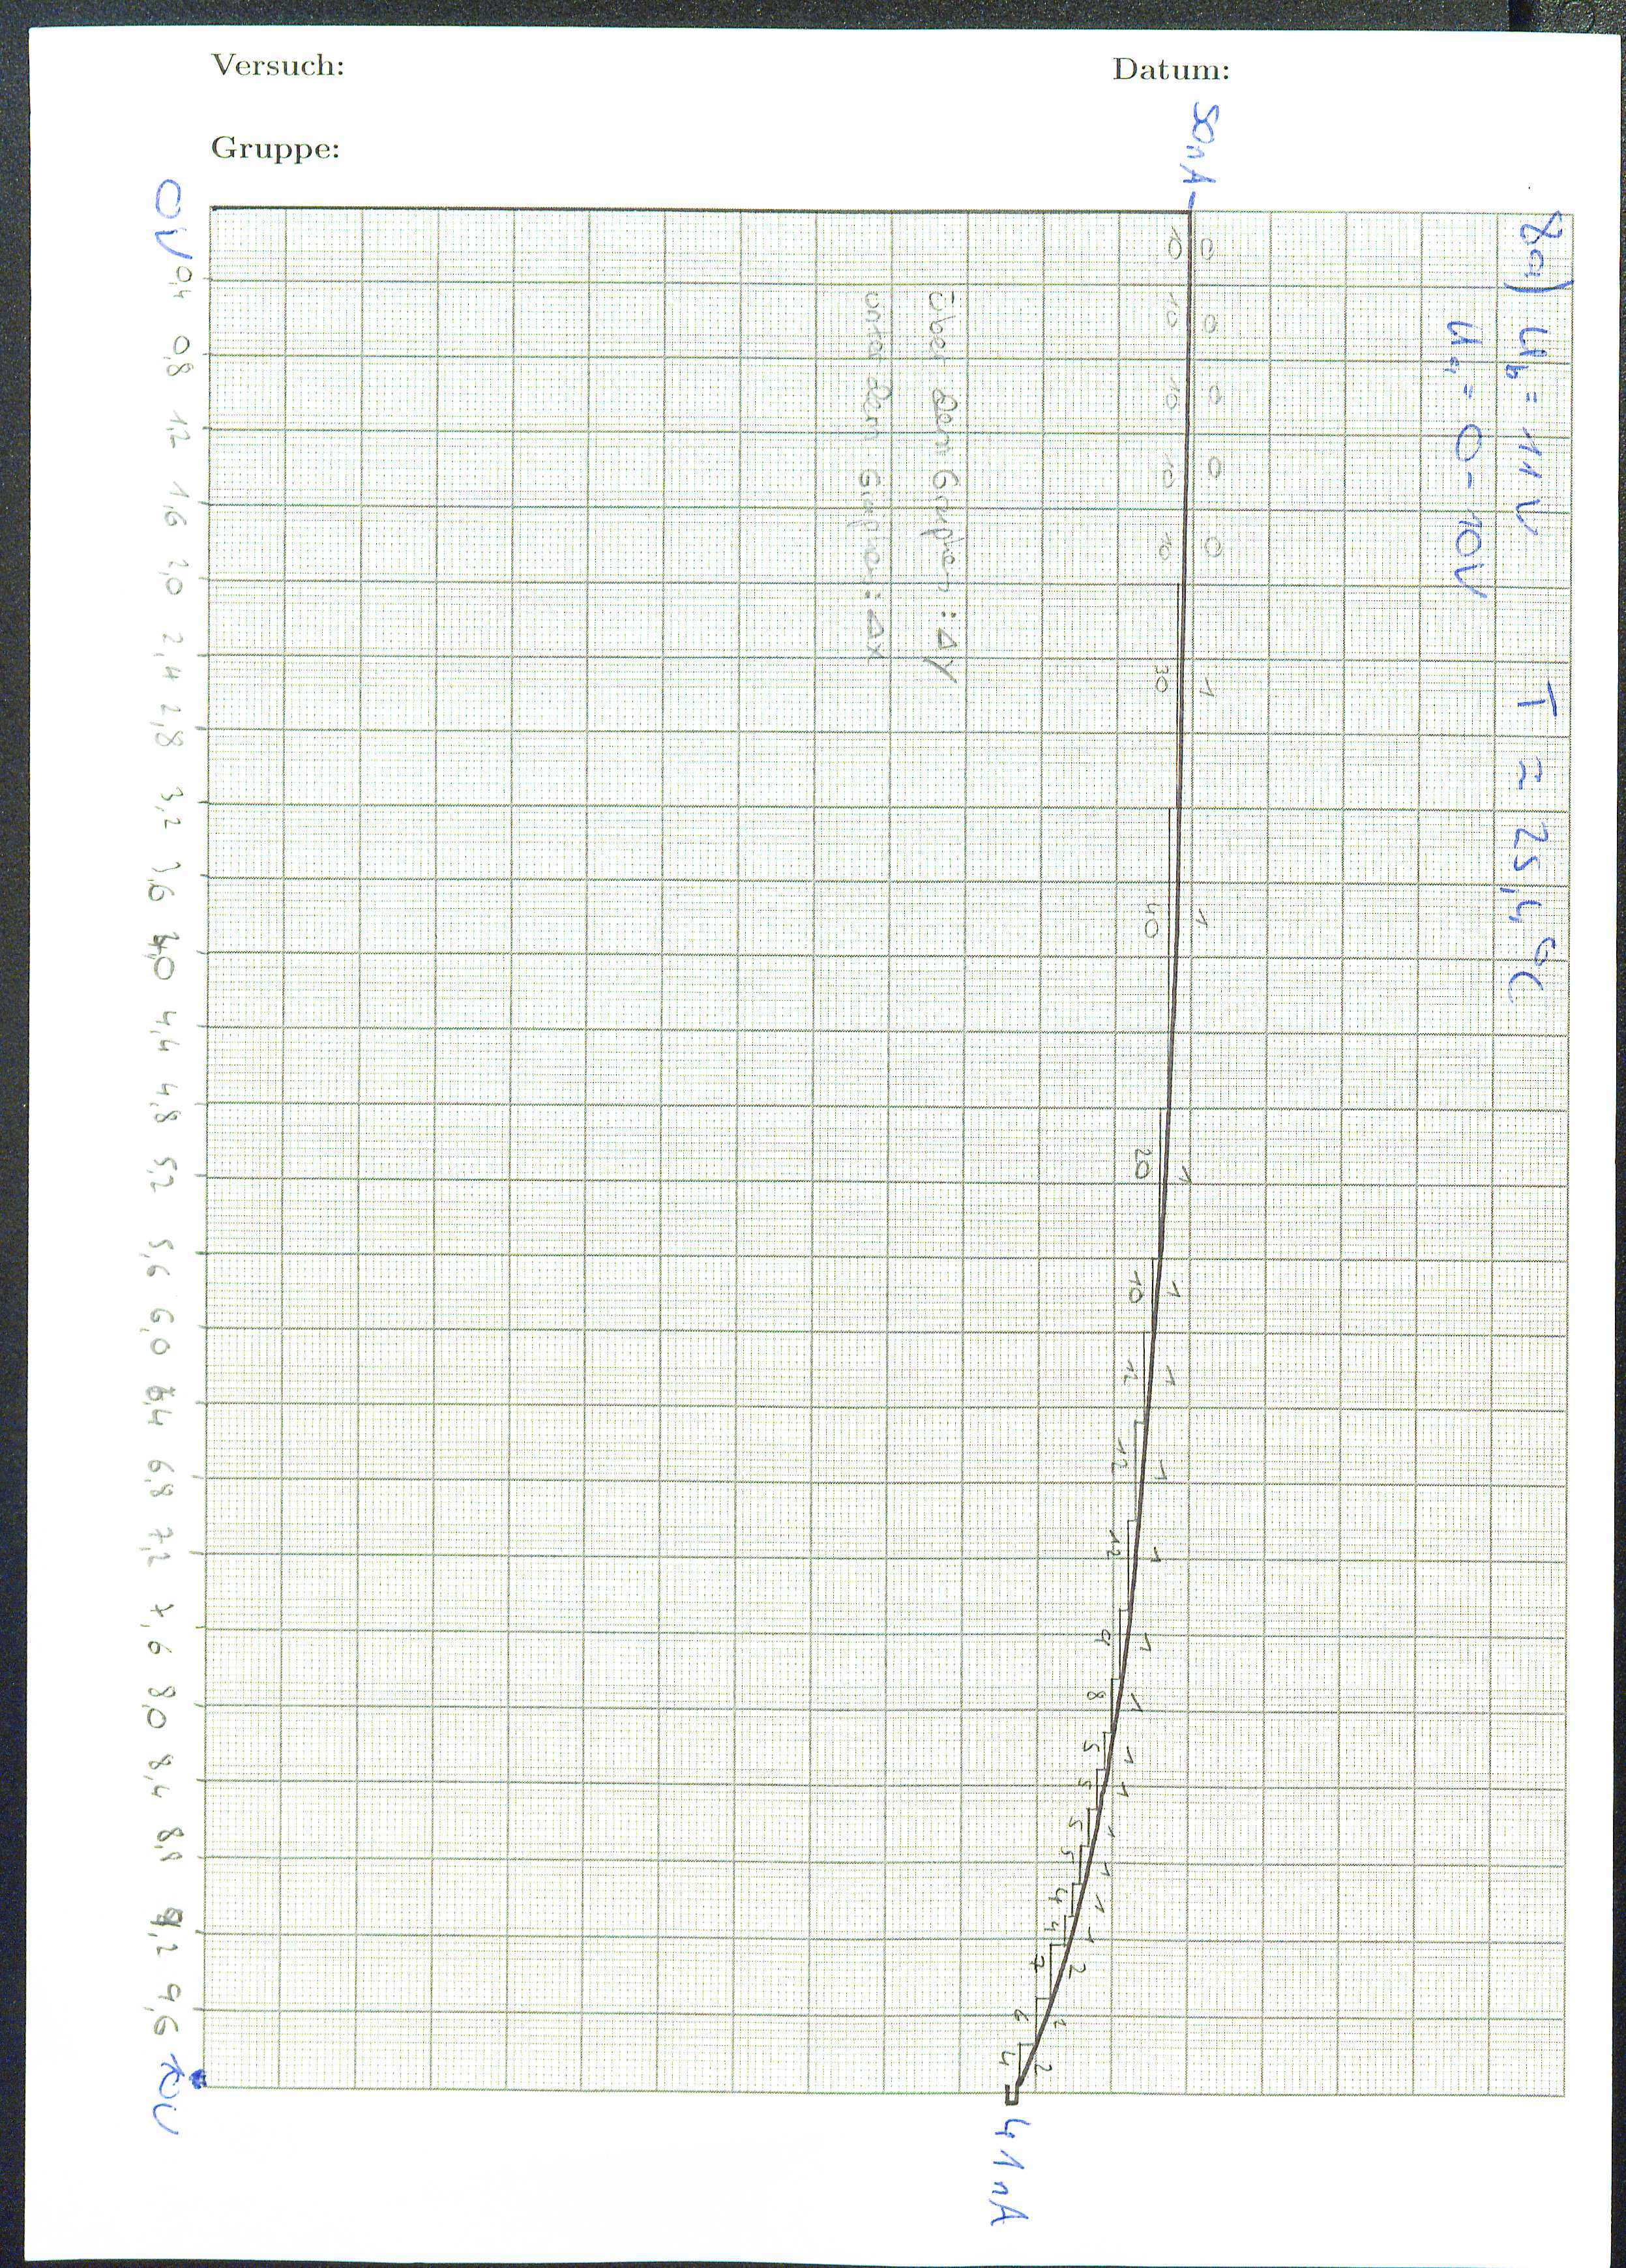
\includegraphics[width=\textwidth]{content/downKurve.jpg}
  \caption{Aufnahme zur Energieverteilung}
  \label{Bild:1}
\end{figure}
\begin{figure}[H]
  \centering
  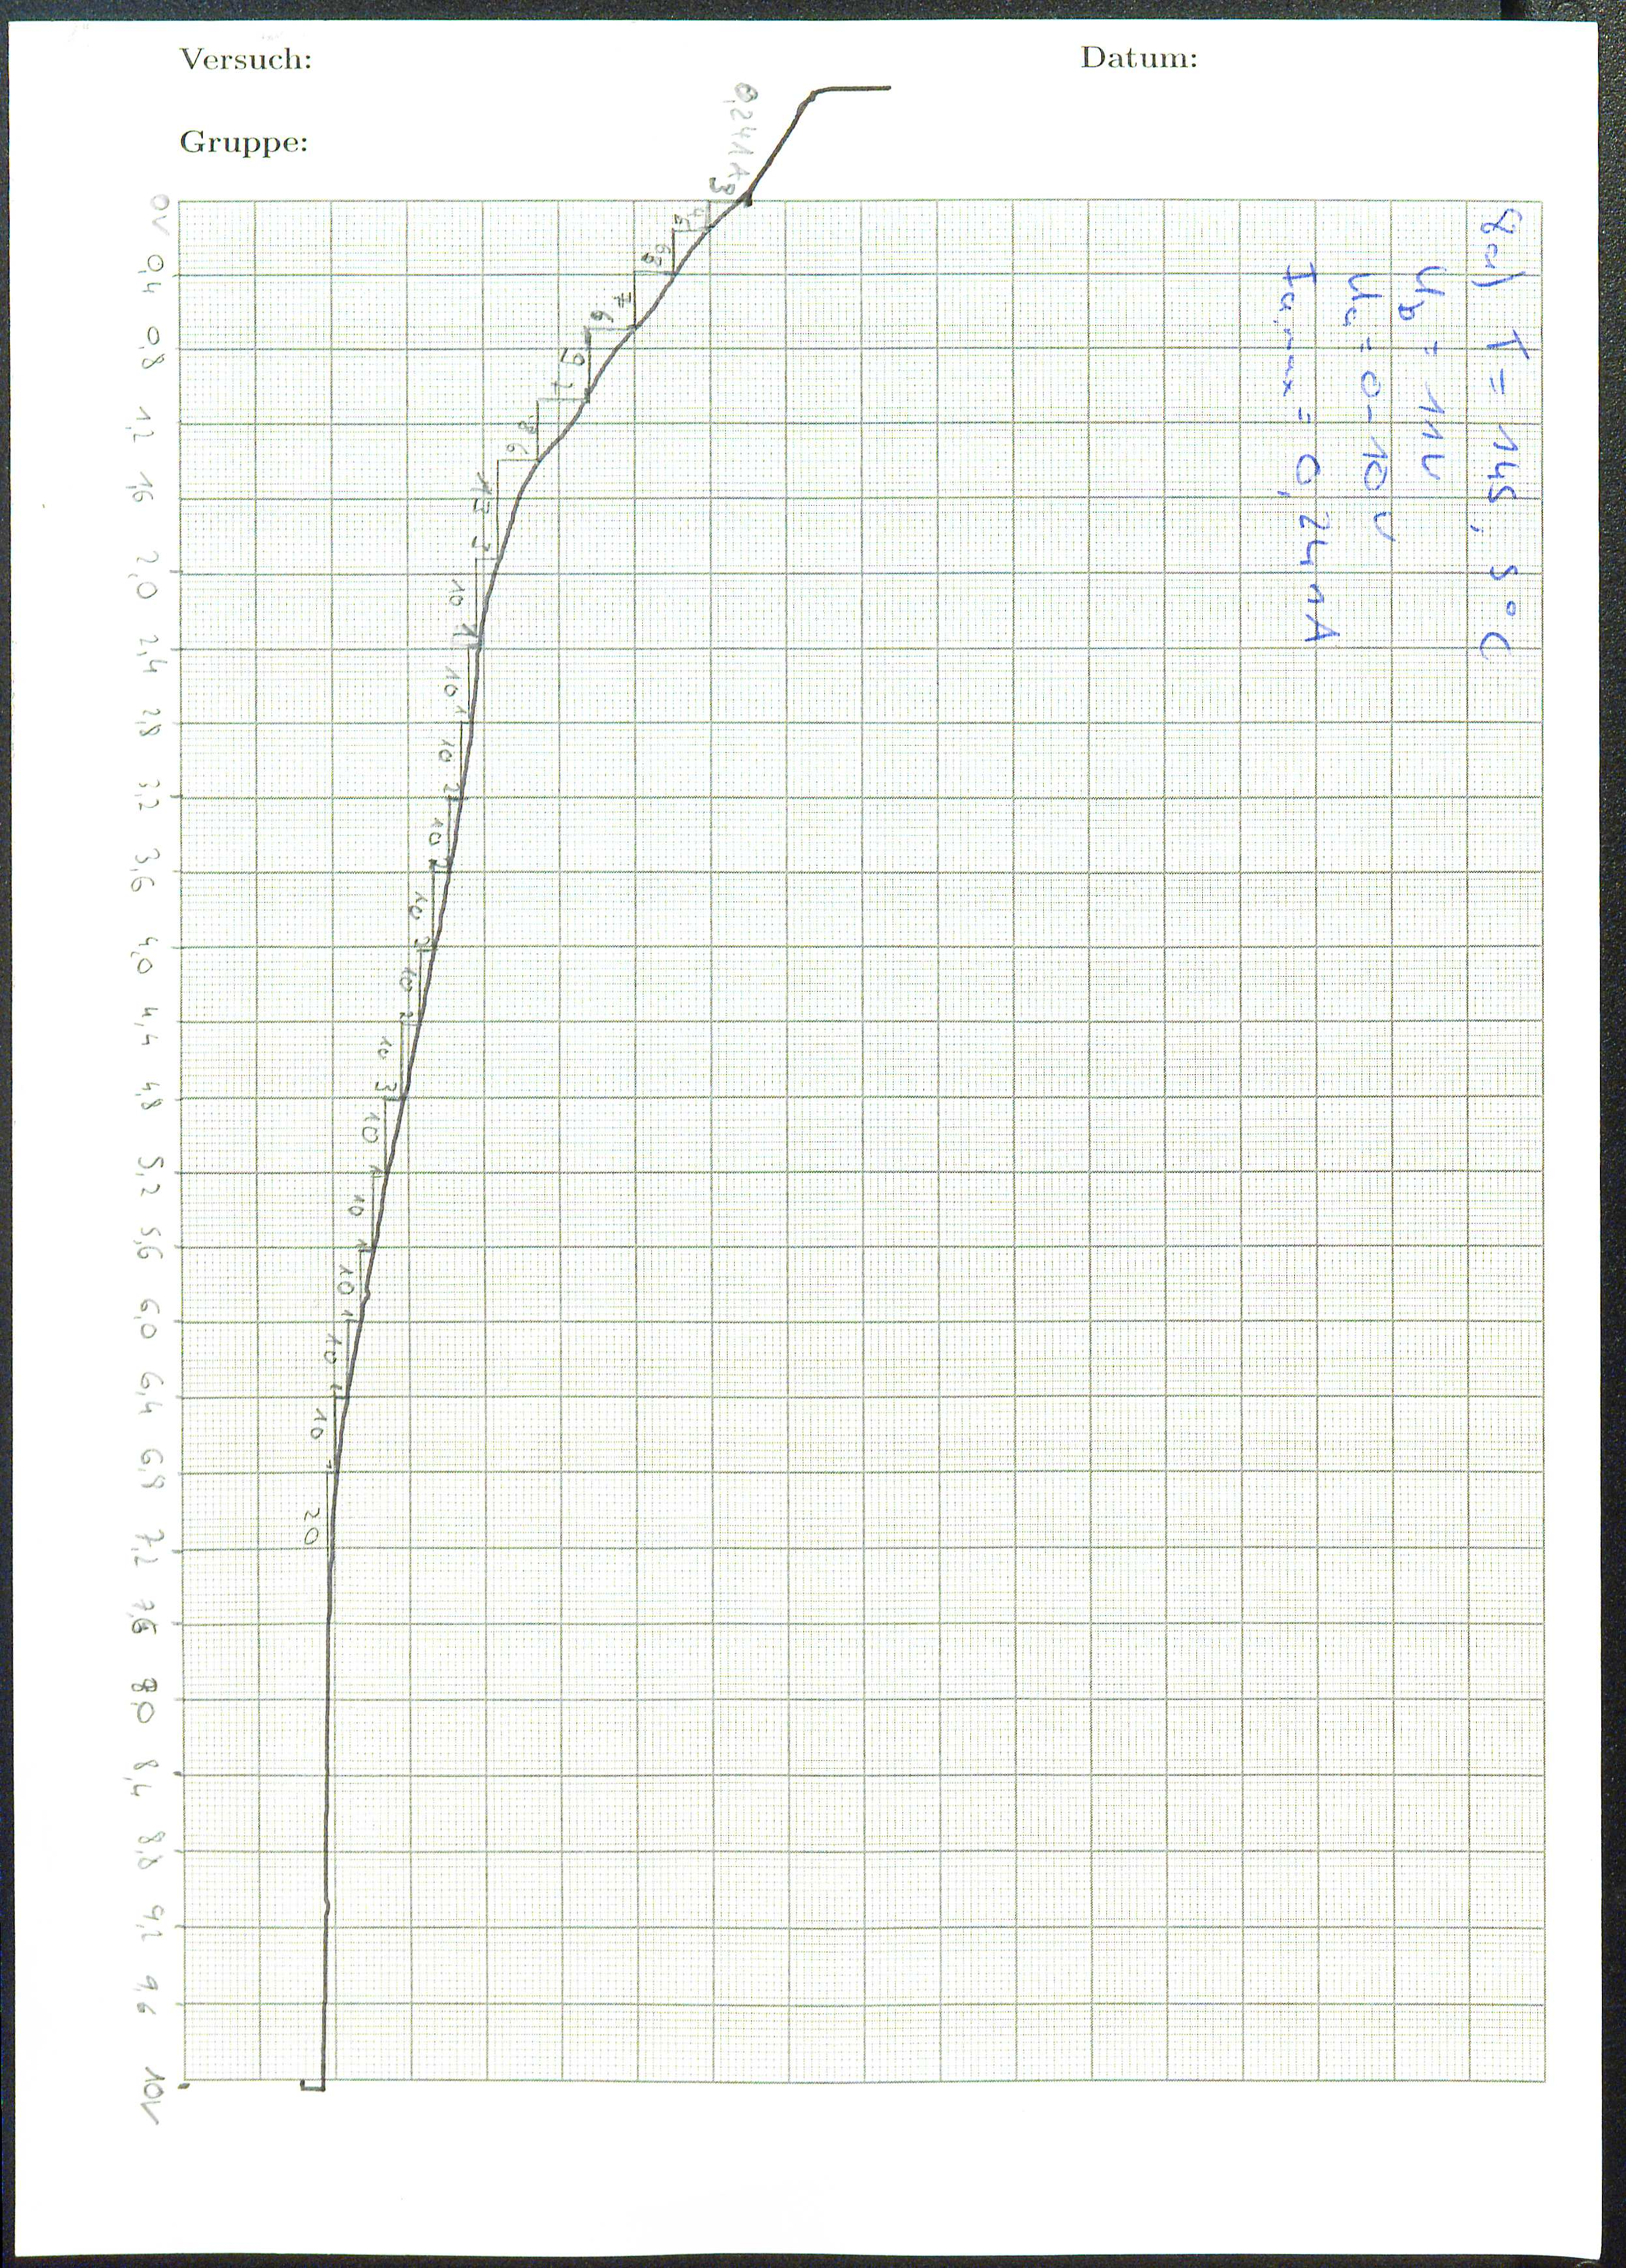
\includegraphics[width=\textwidth]{content/abKurve.jpg}
  \caption{Aufnahme zur Energieverteilung}
  \label{Bild:2}
\end{figure}
\begin{figure}[H]
  \centering
  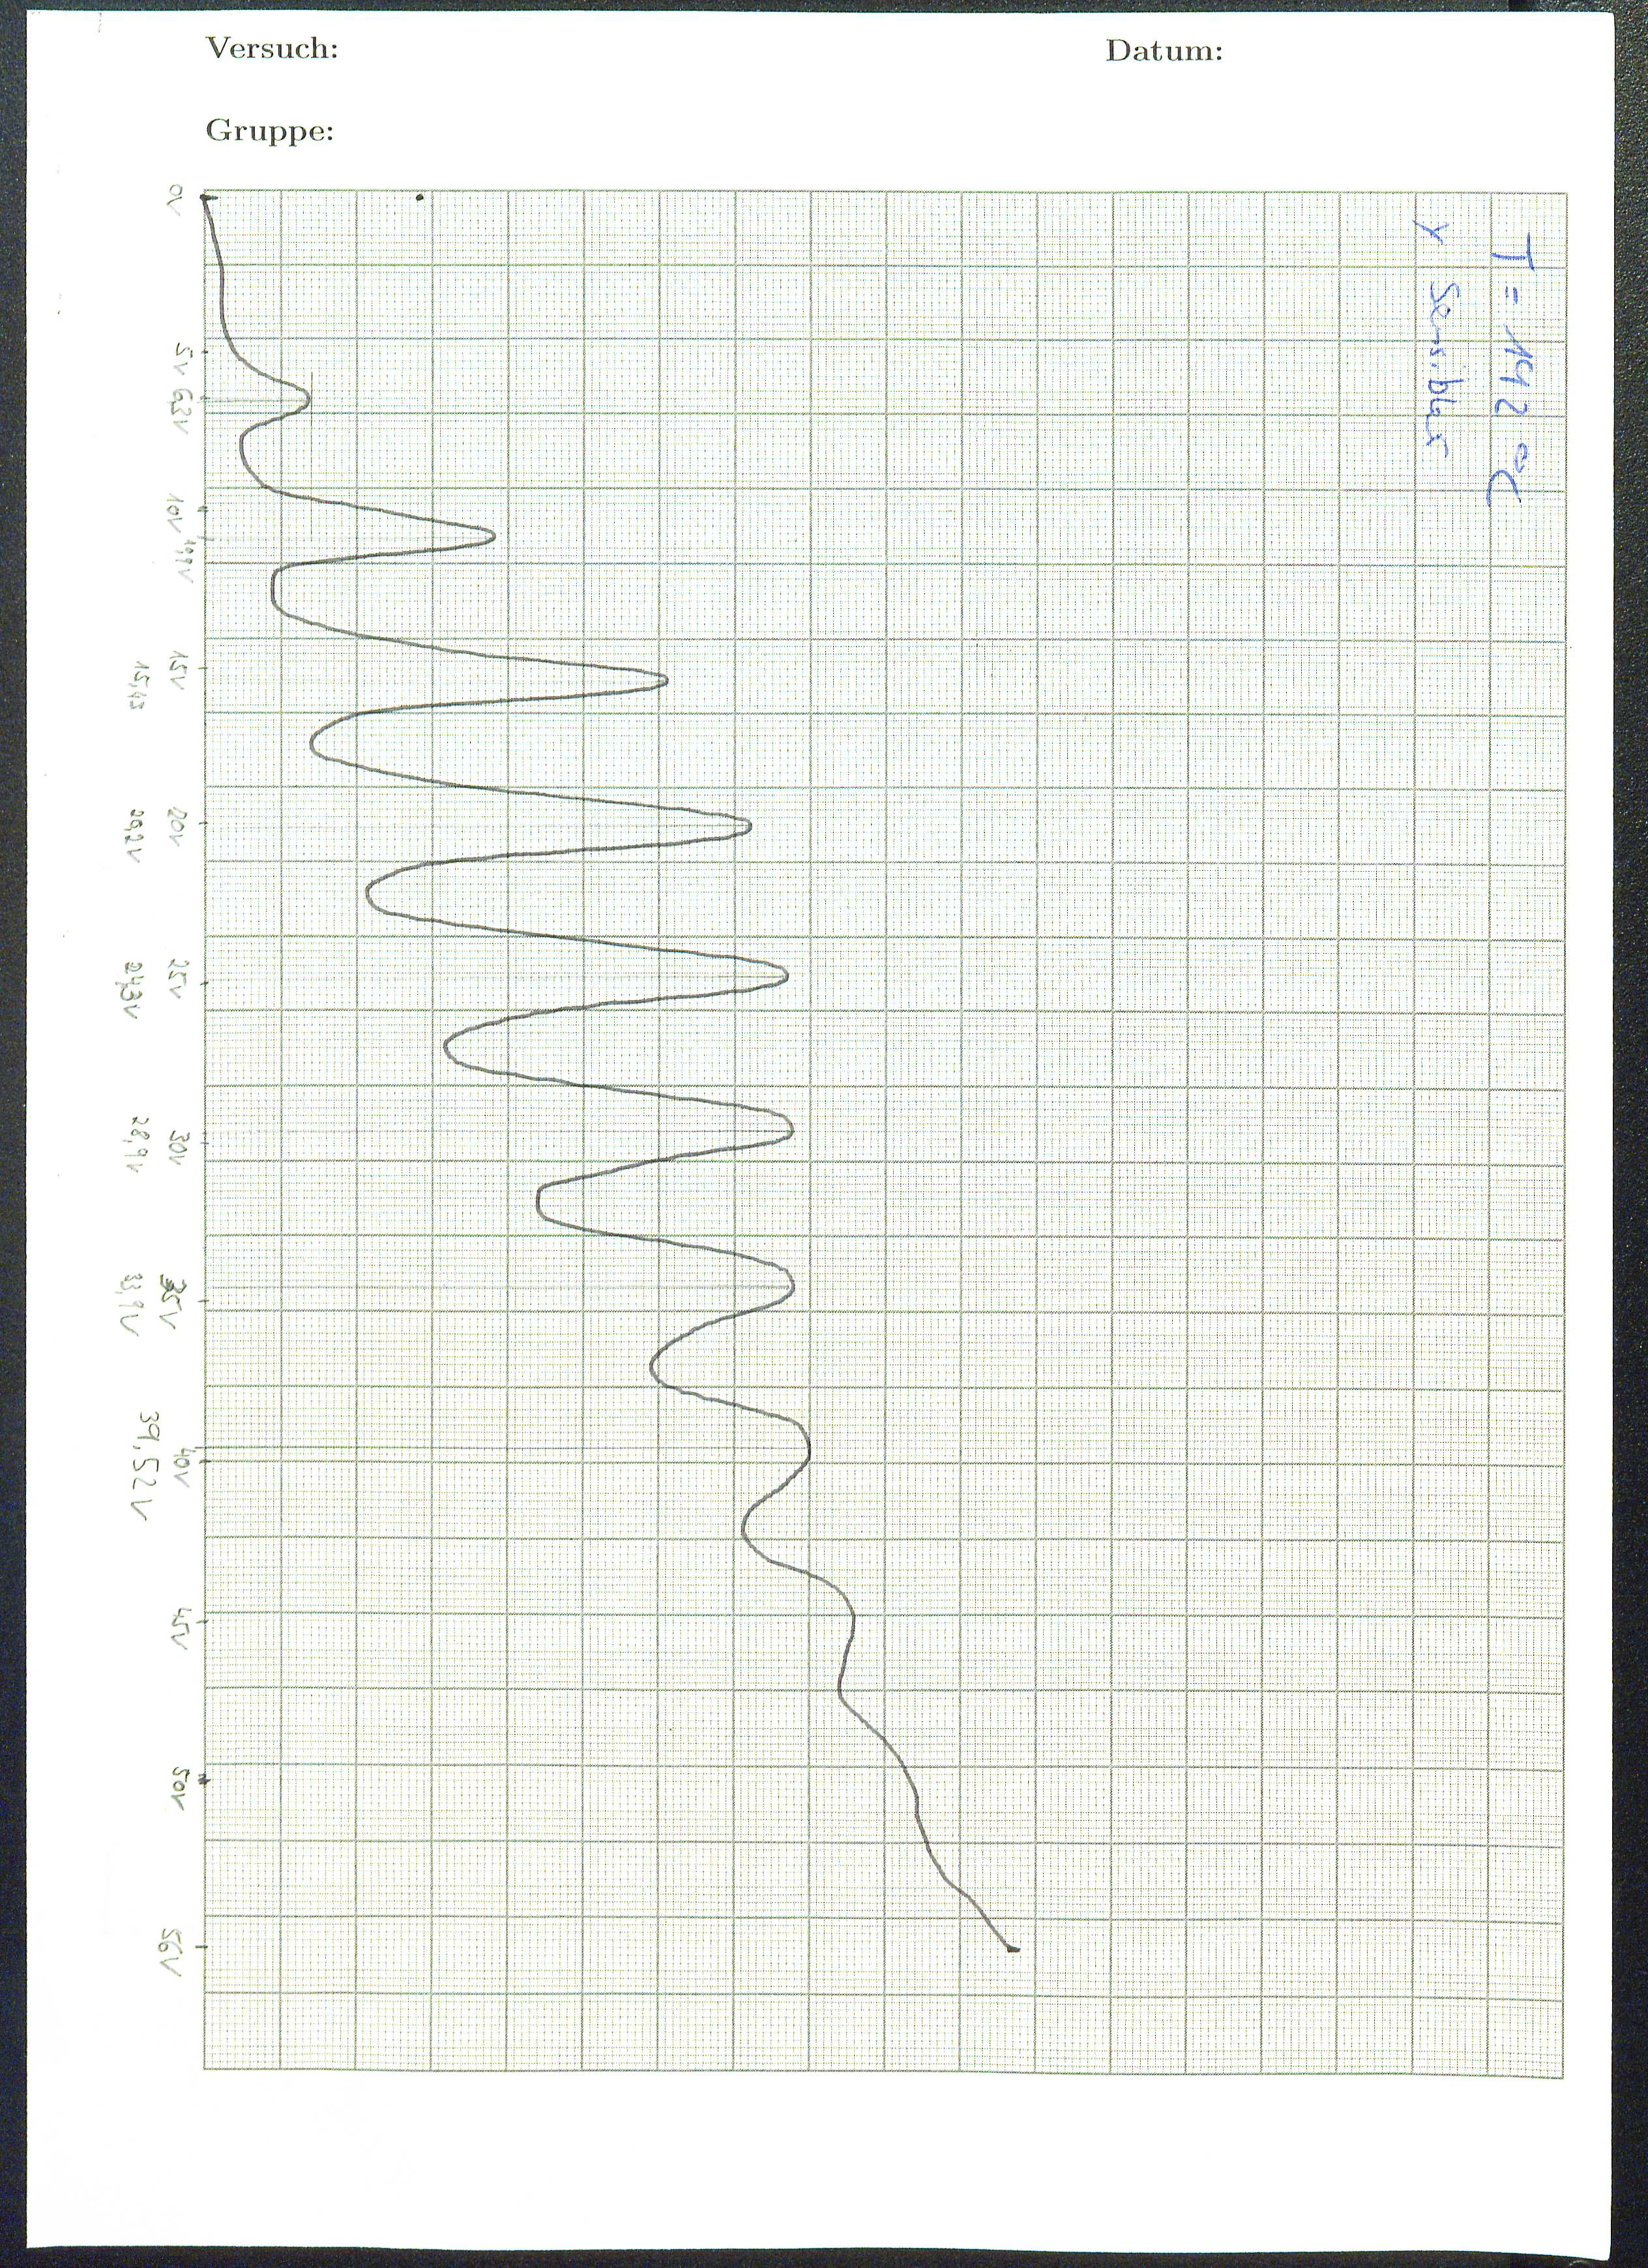
\includegraphics[width=\textwidth]{content/FHKurve.jpg}
  \caption{Aufnahme zur Franck-Hertz-Kurve}
  \label{Bild:3}
\end{figure}
\begin{figure}[H]
  \centering
  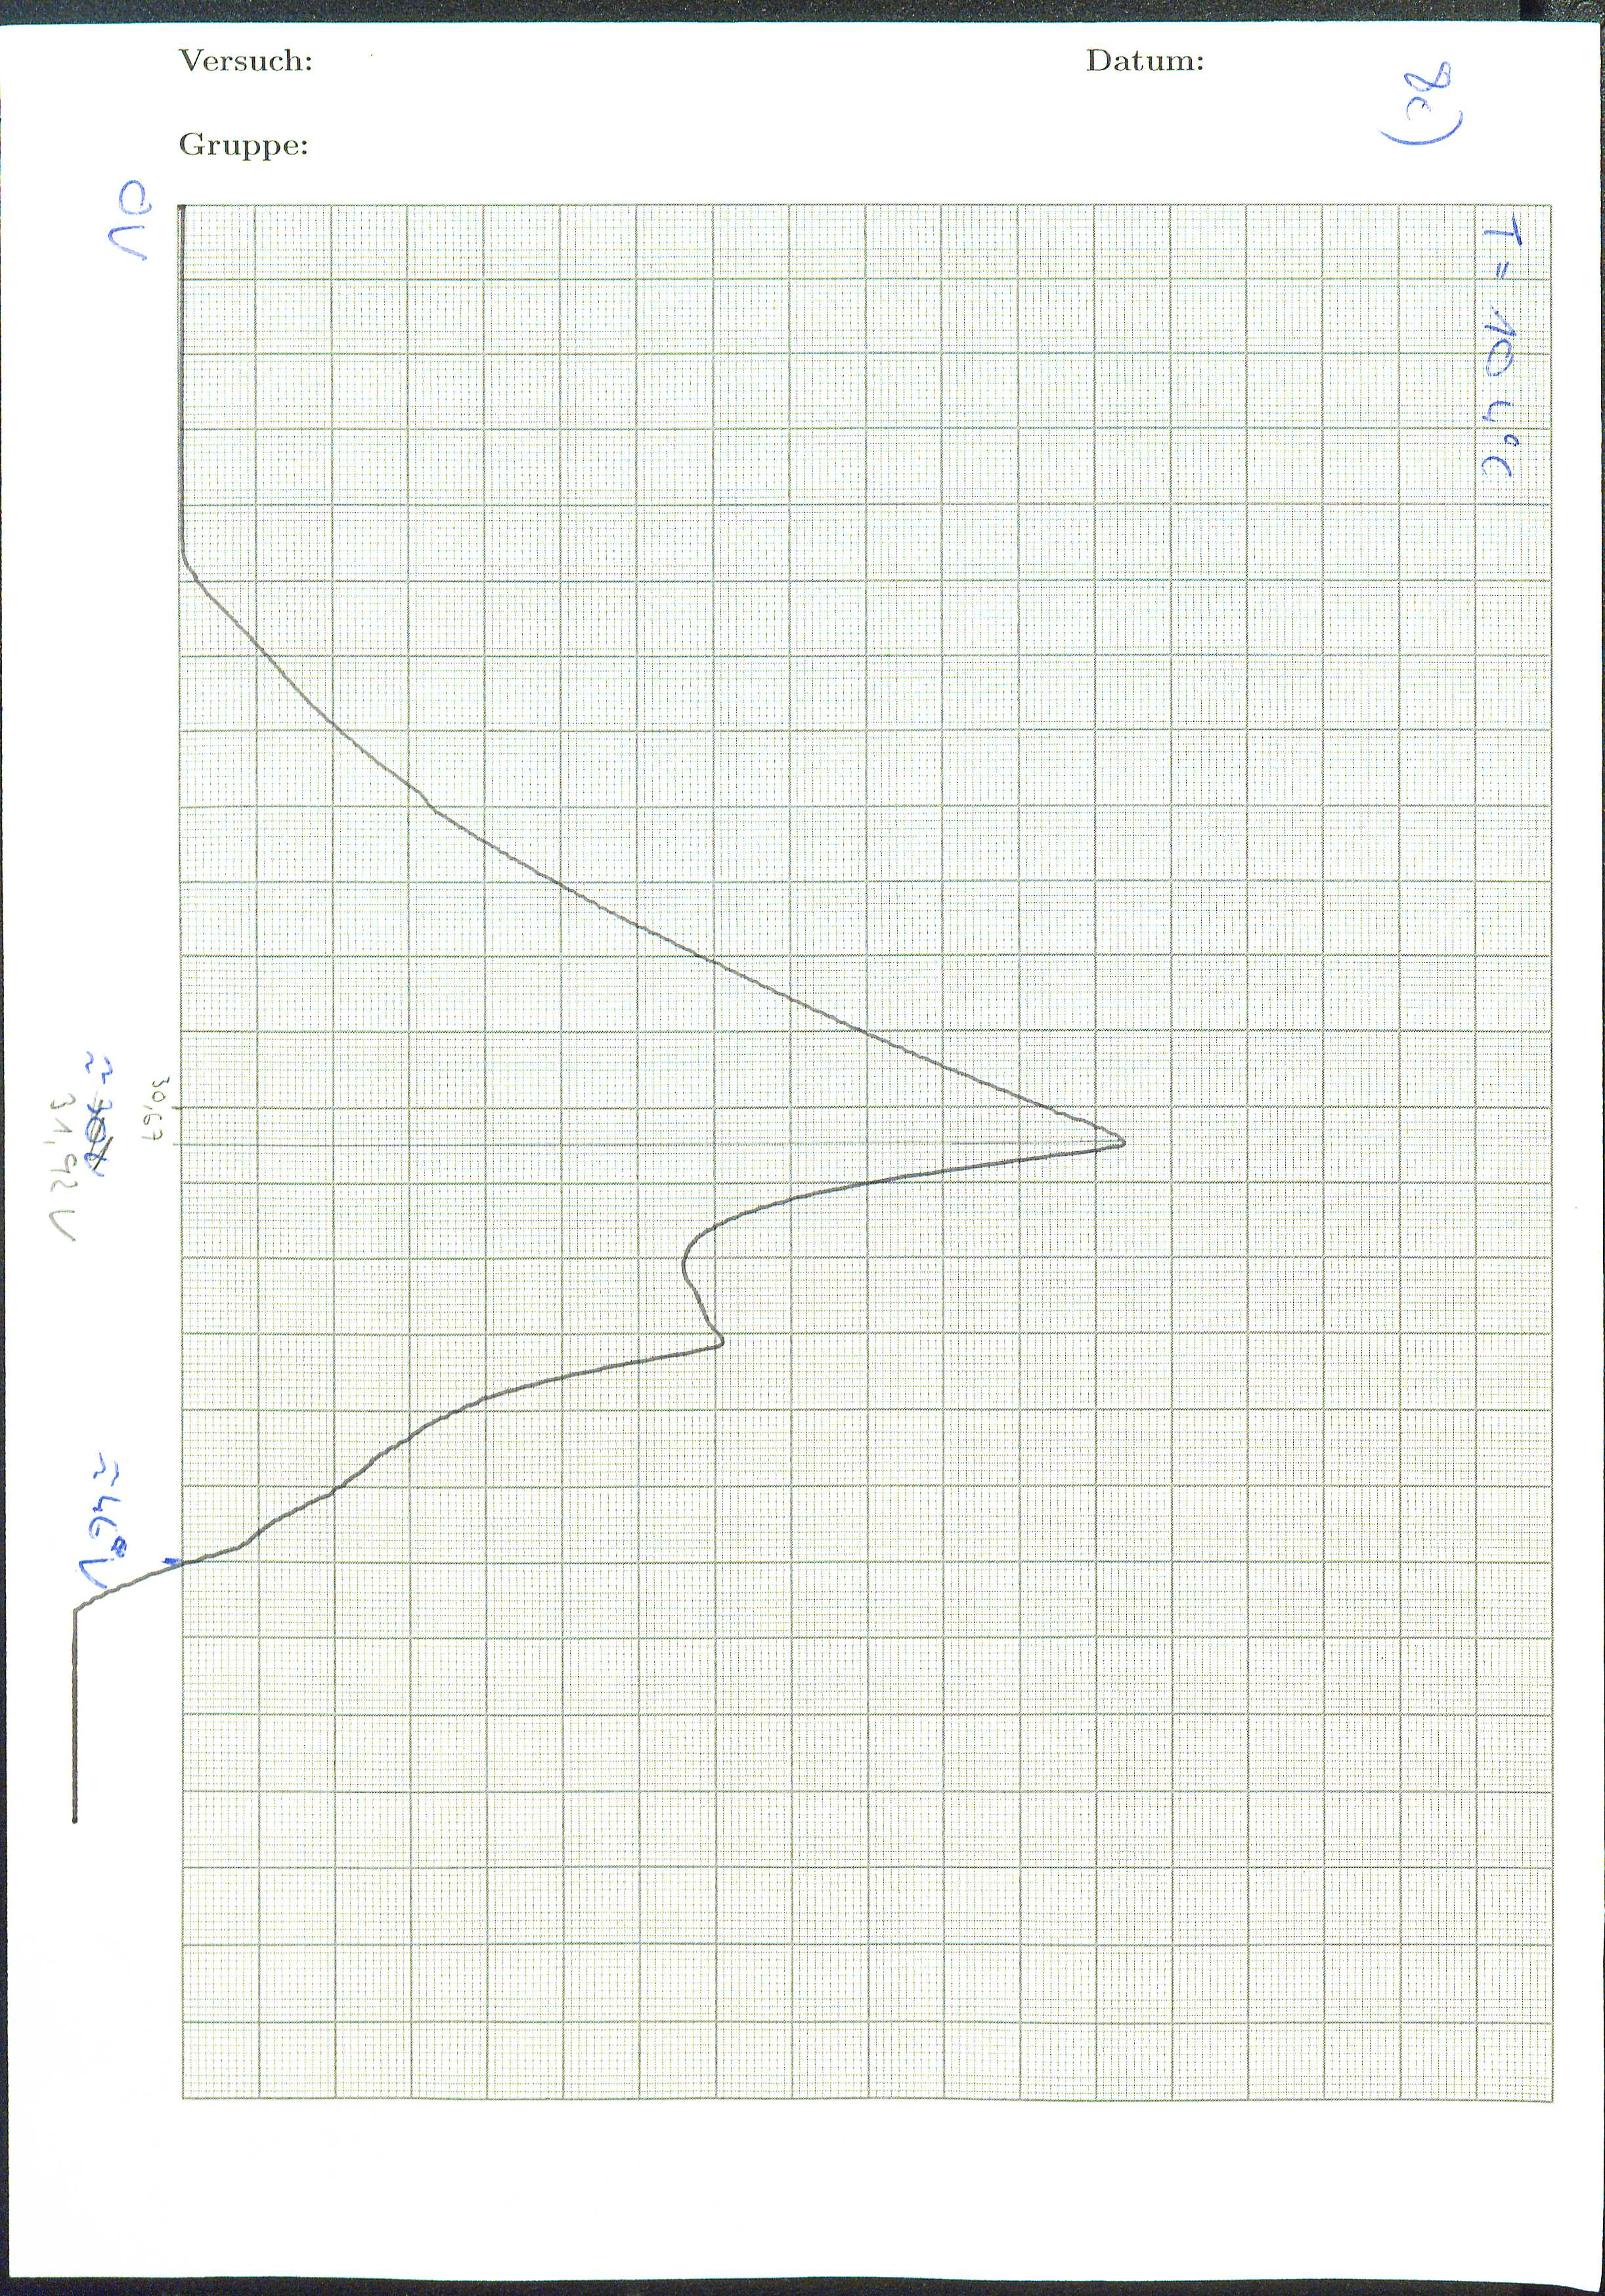
\includegraphics[width=\textwidth]{content/Ionspannung_0001.jpg}
  \caption{Aufnahme zur Bestimmung der Ionisationsenergie}
  \label{Bild:4}
\end{figure}
